% chap2.tex
% 2011/02/03, v1.10

% for multi-contributor books,  use \author
% for single-contributor books, though not required, use \chapterauthor

% uncomment \begin{abstract}...\end{abstract} for the abstract to apppear

  \alphafootnotes
  \author[M\,M Magn\'usson and D\,A Tranah]
    {Magn\'us M\'ar Magn\'usson\footnotemark\
    and David Tranah\footnotemark\\
    International Glaciological Society}

  \chapterauthor{Magn\'us M\'ar Magn\'usson\footnotemark\
    and David Tranah\footnotemark
    \affil{International Glaciological Society}}

  \chapter{The \cambridge\ class file in detail}

  \footnotetext[1]{Formerly of the Icelandic
    Meteorological Office, Reykjav\'\i k.}
  \footnotetext[2]{Supported by NSF Grant 43645.}
  \arabicfootnotes

  \contributor{Magn\'us M\'ar Magn\'usson
    \affiliation{International Glaciological Society,
      Scott Polar Research Institute,
      Lensfield Road, Cambridge CB2 1ER}}

  \contributor{David Tranah
    \affiliation{Cambridge University Press,
      The Edinburgh Building, Shaftesbury Road,
      Cambridge CB2 8RU}}

%\begin{abstract}
%  Thermal convection driven by centrifugal buoyancy in a rapidly rotating narrow annular channel is studied in the case of rigid cylindrical walls.
%\end{abstract}

The following notes may help you achieve the best effects with the \cambridge\ class file.

\section{Frenchspacing}

The \verb"\frenchspacing" option has been selected by default. This ensures that no extra space is inserted after full points, and is normal practice. If there is a strong reason for reversing this, you can key \verb"\nonfrenchspacing" in the preamble.

\section{Adding a subtitle to the front page}

The standard \verb"\title" command has been extended to take an optional argument which is then used as a subtitle on the main title page. For example, this document uses following title command:
\begin{verbatim}
  \title[Subtitle, if you have one]
    {LaTeX2e guide for authors using the \cambridge\ design}
\end{verbatim}


\section{Adding a blank page to your document}

Blank pages should not be numbered. If you require one, use the command \verb"\cleardoublepage", which has been redefined to start the next page on a recto, and if necessary, insert a totally blank verso page first.


\section{Chapter numbering}
If your book starts with an unnumbered chapter (e.g. \verb"\chapter*{Introduction}", then make all the numbered elements (e.g. section heads) unnumbered, by using \verb"\section*{...}". Otherwise, sections will be numbered 0.1, 0.2, etc.

\section{Section numbering}

\LaTeX\ provides five levels of section heads, and they are all defined in the \cambridge\ class file: \verb"\section", \verb"\subsection", \verb"\subsubsection", \verb"\paragraph", and \verb"\subparagraph". Numbers are given for the first three headings.

You can reduce the level of numbered section heads (it is not advisable to increase them). For instance, if you only want headings numbered down to subsections, add the following line to the preamble: \verb"\setcounter{secnumdepth}{2}". To number down to sections, make this \verb"\setcounter{secnumdepth}{1}", etc.


\section{Specifying running heads and toc entries}

\subsection{Single-contributor books}
\label{singlecontributor}

In \cambridge, chapter titles and section heads are used as running heads at the top of every page:
\begin{itemize}
\item chapter titles appear on even-numbered pages (versos), and
\item section heads appear on odd-numbered pages (rectos).
\end{itemize}
A problem with the standard version of \LaTeX\ has always been that the shortened versions of chapter and section titles, specified for running heads, have also been the entries for the toc. There are packages such as the memoir class which enable you to specify different toc entries, running head entries, and chapter titles. However, there is a simple way to add the verbose version of the chapter or section heads into the toc:
\begin{verbatim}
  \chapter[Toc entry]{Verbose chapter title}
  \chaptermark{Running head entry}

  \section[Toc entry]{Verbose section title
    \sectionmark{Running head entry}}
    \sectionmark{Running head entry}
\end{verbatim}
Note that for sections, you need the optional argument to \verb"\section", even if `Toc entry' is in fact the same text as `Verbose section title'. Also, the \verb"\sectionmark" has to be entered twice as shown, because the first \verb"\sectionmark" deals with the header of the page that the \verb"\section" command falls on, and the second deals with subsequent pages.

\subsection{Multi-contributor books}
\label{multicontributor}

Using the \cambridge\ multi-contributor option, author(s) name(s) and chapter titles are used as running heads at the top of every page:
\begin{itemize}
\item author(s) name(s) appear on even-numbered pages (versos), and
\item chapter titles appear on odd-numbered pages (rectos).
\end{itemize}
The author(s) names(s) may run to several lines, and contain new line commands (e.g. \verb"\\"), but the running head must be a single line. To enable you to specify an alternative short form of the author(s) name(s), the standard \verb"\author" command has been extended to take an optional argument to be used as the running head:
\begin{verbatim}
  \author[Author(s) name(s)]{The full author(s) name(s)}
\end{verbatim}
The following shows some coding for a chapter written by two authors, each of whom have footnotes. In this example, the authors' names will immediately follow the chapter title, and will read Magn\'us M\'ar Magn\'usson$^{a}$ and David Tranah$^{b}$. Their respective footnotes will be `$^{a}\enskip$Formerly of the Icelandic Meteorological Office, Reykjav\'\i k.' and `$^{b}\enskip$Supported by NSF~Grant 43645.' It is crucial that \verb"\author" precedes \verb"\chapter". If the authors have footnotes, you must start the chapter with \verb"\alphafootnotes", fill in the details for author(s), chapter title and author footnotes, then key \verb"\arabicfootnotes" to revert to arabic footnotes:
\begin{verbatim}
  \alphafootnotes
  \author[M\,M Magn\'usson and D\,A Tranah]
    {Magn\'us M\'ar Magn\'usson\footnotemark\
    and David Tranah\footnotemark\\
    International Glaciological Society}

  \chapter[Running head entry]
    {The \cambridge\ class file in detail}

  \footnotetext[1]{Formerly of the Icelandic
    Meteorological Office, Reykjav\'\i k.}
  \footnotetext[2]{Supported by NSF Grant 43645.}
  \arabicfootnotes
\end{verbatim}
Note that for multi-contributor books, the long version of the chapter title will always appear in the table of contents.


\section{Adding author(s) name(s) in single-contributor books}
Sometimes, chapters in single-contributor books are written by different people. If you wish the authors (and their affiliations) to appear beneath the chapter opening, as demonstrated in this chapter, key your chapter head as follows; note that \verb"\chapterauthor" must precede \verb"\chapter":
\begin{verbatim}
  \alphafootnotes
  \chapterauthor{Magn\'us M\'ar Magn\'usson\footnotemark\
    and David Tranah\footnotemark
    \affil{International Glaciological Society}}

  \chapter{The \cambridge\ class file in detail}

  \footnotetext[1]{Formerly of the Icelandic
    Meteorological Office, Reykjav\'\i k.}
  \footnotetext[2]{Supported by NSF Grant 43645.}
  \arabicfootnotes
\end{verbatim}
If you have footnotes associated with the authors, you will also need to insert \verb"\alphafootnotes" and \verb"\arabicfootnotes".

\section{List of contributors}
\label{contrib}
The code for generating an automatic list of contributors should be entered after the author and chapter titles, as follows:
\begin{verbatim}
  \contributor{Magn\'us M\'ar Magn\'usson
    \affiliation{International Glaciological Society,
      Scott Polar Research Institute,
      Lensfield Road, Cambridge CB2 1ER}}

  \contributor{David Tranah
    \affiliation{Cambridge University Press,
      The Edinburgh Building, Shaftesbury Road,
      Cambridge CB2 8RU}}
\end{verbatim}
You then simply need to add the \verb"\listofcontributors" command after the table of contents (or after the artwork lists, if included) in the preamble, as follows:
\begin{verbatim}
  \tableofcontents
  \listoffigures
  \listoftables
  \listofcontributors
\end{verbatim}

\subsection{Note to editors regarding the list of contributors}

The contributors will appear in the same order as they are called in, since the list is generated in the same way as the table of contents. This means that at the final stage, the file will require editing to make the entries alphabetic.

Once you have a complete list of contributors, comment out the line which is generating them, and replace it as shown below:
\begin{verbatim}
  \tableofcontents
  \listoffigures
  \listoftables
 %\listofcontributors
  \editedlistofcontributors
\end{verbatim}
Next, rename the file with the extension \verb".loc" to \verb"editedloc.tex" (in the case of this guide, you would rename \texttt{\cambridge guide.loc} to \verb"editedloc.tex"). Edit this file as required, then run the file through \LaTeX\ once more, and the edited version will appear.

\section{Adding an abstract}
The following code will give you an unnumbered section head `Abstract'. Keep the abstract to one paragraph:
\begin{verbatim}
  \begin{abstract}
    Thermal convection driven by centrifugal...
  \end{abstract}
\end{verbatim}

\section{Adding an extract}
You may add an extract -- the following coding:
\begin{verbatim}
  \begin{extract}
    In a semiparametric model, some aspects of the data
    distribution are specified in terms of a small number of
    parameters, but other aspects are left arbitrary.
  \end{extract}
\end{verbatim}
will produce:
  \begin{extract}
    In a semiparametric model, some aspects of the data
    distribution are specified in terms of a small number of
    parameters, but other aspects are left arbitrary.
  \end{extract}

\section{Adding a `copyright' line to a chapter opening~page}
If you are publishing a single chapter, with permission from Cambridge University Press, you may be required to add a copyright line (and/or other information) to the footer of the chapter opening page. This may be achieved using:
\begin{verbatim}
  \copyrightline{Reprinted from \textit{Mathematical
    Methods for Physics and Engineering} by Riley,
    Hobson and Bence \copyright\ 2009 Cambridge
    University Press.}
\end{verbatim}
Should the following chapter not require the copyright line, reverse this immediately before the next \verb"\chapter" command by using:
\begin{verbatim}
  \copyrightline{}
\end{verbatim}


\section{Changing the level of entries in the table of~contents}
\label{changingentries}
The \cambridge\ design will, by default, list parts, chapters and sections in the table of contents. However, to improve the usefulness of this guide, we have used the command:
\begin{verbatim}
  \setcounter{tocdepth}{2}
\end{verbatim}
to increase this by one level, so the table of contents in this document also shows subsections.


\section{Lists}
\label{lists}

The \cambridge\ class provides the following standard list environments:
\begin{enumerate}
 \item numbered lists, created using the \verb"enumerate" environment;
 \item bulleted lists, created using the \verb"itemize" environment;
 \item labelled lists, created using the \verb"description" environment.
\end{enumerate}
The \verb"enumerate" environment numbers each list item with an arabic numeral followed by a full point; alternative styles can be achieved by inserting a redefinition of the number labelling command after the \verb"\begin{enumerate}". For example, a list numbered with lower-case letters inside parentheses can be produced. Because `(a)' is wider than a standard arabic digit, the label width has to be increased. This is achieved by specifying the widest label in the list inside square braces:
\begin{verbatim}
  \begin{enumerate}[(a)]
    \renewcommand{\theenumi}{(\alph{enumi})}
    \item estimate the fluctuations in the near-wall region\ldots
    \item subdue these near-wall fluctuations\ldots
  \end{enumerate}
\end{verbatim}
This produces the following list:
  \begin{enumerate}[(a)]
    \renewcommand{\theenumi}{(\alph{enumi})}
    \item estimate the fluctuations in the near-wall region\ldots
    \item subdue these near-wall fluctuations\ldots
  \end{enumerate}


\section{Endnotes}

In addition to footnotes,\footnote{The footnote counter will be reset on chapters.} the \cambridge\ class provides a similar facility for endnotes. Their appearance depends on which option you are using:
\begin{enumerate}
\item for single-contributor books, the endnotes will be produced in the form of an unnumbered chapter at the end of the book;
\item for multi-contributor books, they are an unnumbered section at the end of each chapter.
\end{enumerate}
Endnotes are inserted into the text in a similar way to footnotes, but using the \verb"\endnote" command; for example,
\begin{verbatim}
  When the Richardson number\endnote{Lewis Fry Richardson
  (1881--1953).\label{richardson}} increases\ldots
\end{verbatim}
will produce `When the Richardson number\endnote{Lewis Fry Richardson (1881--1953).\label{richardson}} increases\ldots' in the text. Authors must choose between using footnotes and endnotes; do not use both.

\subsection{Single-contributor books}
Endnotes should be printed at the end of the book, after the appendices but before the bibliography and/or references.
\begin{verbatim}
    :
  \theendnotes
  \begin{thebibliography}{99}
    :
\end{verbatim}
The \verb"\theendnotes" command generates an unnumbered chapter which appears in the table of contents (see page~\pageref{richardson} for style).

\subsection{Multi-contributor books}

Endnotes should be printed at the end of the chapter using the same \verb"\theendnotes" command.

\section{Examples}
\label{examples}
Examples have rules both above and below. If you require two or more to appear together, simply add another \verb"\item" within the \verb"examplelist" environment (e.g. Example~\ref{fourier}):
\begin{verbatim}
  \begin{examplelist}
    \item Show that the geometrical definition of grad leads to the
          usual expression for $\nabla\phi$ in Cartesian coordinates.
    \solution
          Consider a small rectangular volume element $\Delta V =
          \Delta x\,\Delta y\,\Delta z$ with its faces parallel to the
          $x,y,z$ coordinate surfaces and with the point $P$ at one
          corner. We must calculate\ldots

    \item Find the Fourier series of $f(x) =  x^3$ for $0 < x \leq 2$.
    \label{fourier}
    \solution
          In the example discussed in the previous section we found
          the Fourier series for $f(x) = x^2$ in the required range.
          So, if we \textit{integrate} this term by term\ldots
  \end{examplelist}
\end{verbatim}
This will produce:
  \begin{examplelist}
    \item Show that the geometrical definition of grad leads to the
          usual expression for $\nabla\phi$ in Cartesian coordinates.
    \solution
          Consider a small rectangular volume element $\Delta V =
          \Delta x\,\Delta y\,\Delta z$ with its faces parallel to the
          $x,y,z$ coordinate surfaces and with the point $P$ at one
          corner. We must calculate\ldots

    \item Find the Fourier series of $f(x) =  x^3$ for $0 < x \leq 2$.
    \label{fourier}
    \solution
          In the example discussed in the previous section we found
          the Fourier series for $f(x) = x^2$ in the required range.
          So, if we \textit{integrate} this term by term\ldots
  \end{examplelist}


\section{Problems}

Authors may use the \verb"problemlist" environment which will typeset problems at the end of each section or chapter. This is shown in the following example:
\begin{verbatim}
  \begin{problemlist}
    \item Show that the link between shock formation and
          film rupture is invoked here because of the\ldots
    \item Show that the physical interpretation of\ldots
          \label{physi}
  \end{problemlist}
\end{verbatim}
which will produce:
  \begin{problemlist}
    \item Show that the link between shock formation and
          film rupture is invoked here because of the\ldots
    \item Show that the physical interpretation of\ldots
          \label{physi}
  \end{problemlist}
As with all numbered environments, individual problems (e.g. Problem~\ref{physi}) may be cross-referenced.


\section{Boxes}

Boxes may be typeset using the following coding. They are effectively floats, and so can take the optional arguments [h], [t], [b], as used for figures and tables. The following coding produces Box~\ref{fb}:
\begin{verbatim}
  \begin{floatingbox}[h]
    \caption{Floating box title}
      There are grounds for cautious optimism that we may now
      be near the end of the search for the ultimate laws of
      nature -- Stephen Hawking
    \label{fb}
  \end{floatingbox}
\end{verbatim}
  \begin{floatingbox}[h]
    \caption{Floating box title}
      There are grounds for cautious optimism that we may now
      be near the end of the search for the ultimate laws of
      nature -- Stephen Hawking
    \label{fb}
  \end{floatingbox}

\section{Figures}

The \cambridge\ class file will cope with most positioning of your figures. As captions normally fall below figures, the figure must be included first, then the caption, then the label. This is illustrated in Figure~\ref{cantor}. The \verb"cantor1.eps" file has been called in by using \verb"\usepackage{graphicx}" in the preamble. Note that if you are producing a list of illustrations (using \verb"\listoffigures"), you need to repeat the caption in square braces, but without the full point.

\subsection{Figures between two-thirds and full text width}

If the width of the figure lies between two-thirds and the full text width (in other words, between 19pc and 29pc), the figure may be typeset using standard \LaTeX\ coding (see Figure~\ref{cantor}).

  \begin{figure}
    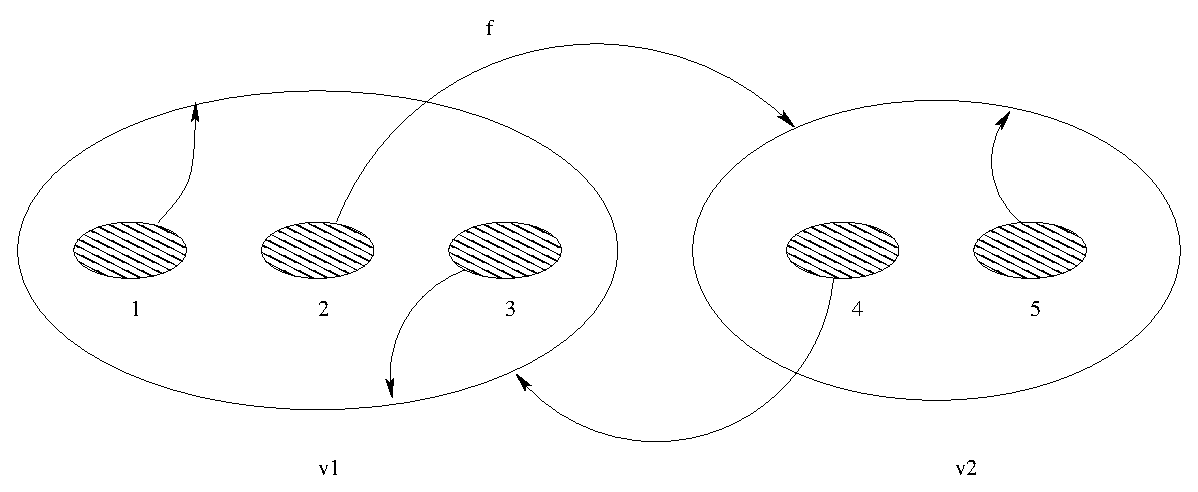
\includegraphics[width=\textwidth]{cantor1.eps}
    %  note that the square brace option below is only required
    %  if you intend to produce a list of illustrations
    \caption[Shortened figure caption for the list of illustrations]
      {A Cantor repeller. Figure captions will be left-aligned,
      29pc wide, and unjustified.}
    \label{cantor}
\rule[-20pt]{\textwidth}{0.5pt}
\begin{verbatim}
  \begin{figure}
    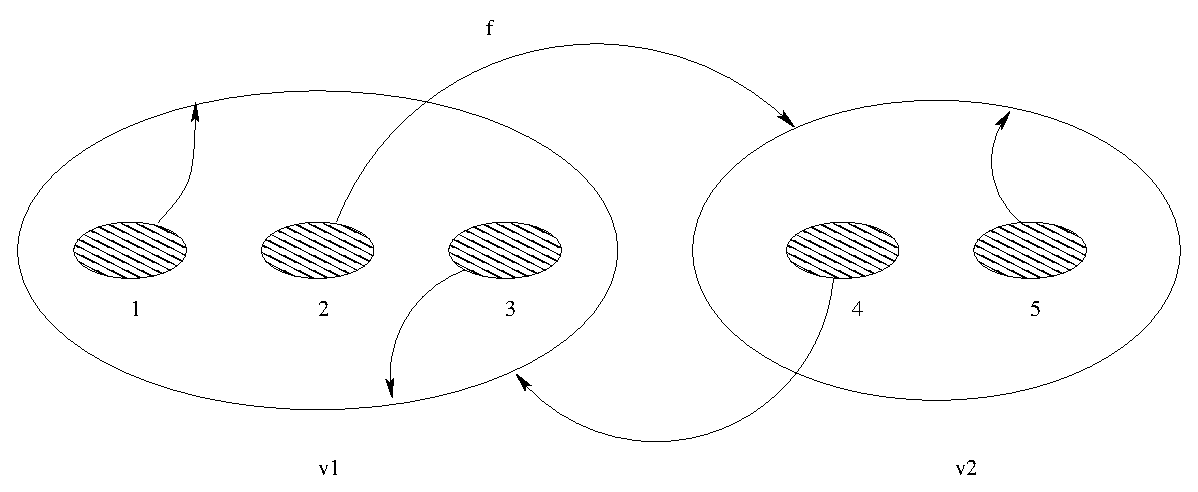
\includegraphics[width=\textwidth]{cantor1.eps}
    %  note that the square brace option below is only required
    %  if you intend to produce a list of illustrations
    \caption[Shortened figure caption for the list of illustrations]
      {A Cantor repeller. Figure captions will be left-aligned,
      29pc wide, and unjustified.}
    \label{cantor}
  \end{figure}
\end{verbatim}
\rule[20pt]{\textwidth}{0.5pt}
  \end{figure}

\subsection{Figures less than two-thirds of the text width}

If you have a figure which takes up less than two-thirds of the text width, i.e. less than 19pc, you have two options. You may either have the caption below the figure, or choose the space-saving option of placing it to the side.

\subsubsection{Caption below figure}

In this case, you would use the \verb"figure" environment (see Figure~\ref{cantor}) and size your figure accordingly.

\subsubsection{Caption to the side of figure}
\label{captiontoside}

To typeset the figure caption to the side, we recommend using the \verb"sidecap" style file; for coding see Figure~\ref{scfigure}. Note that the \verb"[50]" option on the first line will make the caption extend to the full width of the page, and is therefore essential.

Should you have a long caption which extends below the figure, you will need to revert to the \verb"figure" environment.
%
%  \begin{SCfigure}[50]
%    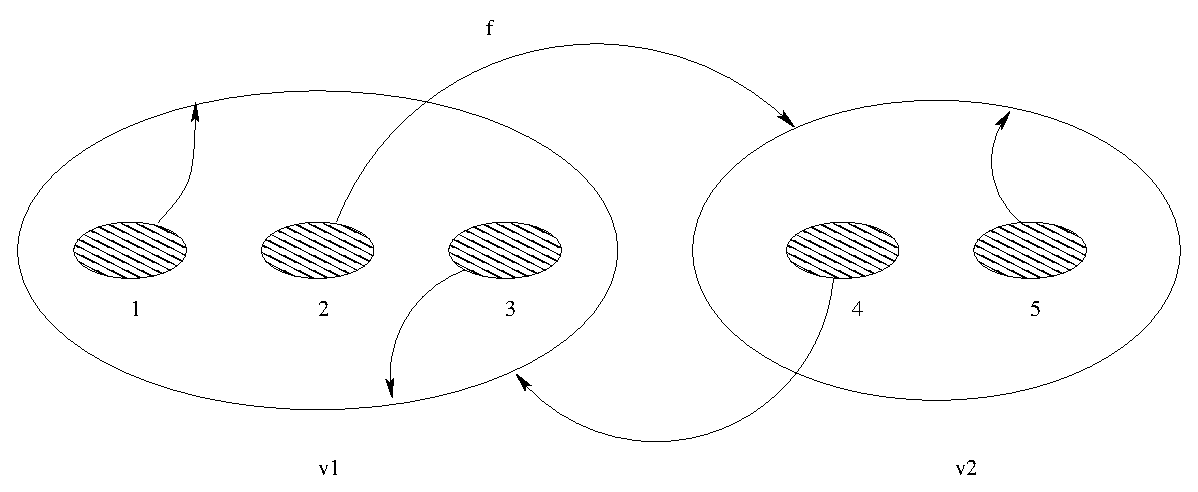
\includegraphics[width=18pc]{cantor1.eps}
%      \caption[Figure with side caption]
%        {The \texttt{SCfigure} environment should be used if you
%          would like a side caption.}
%      \label{scfigure}
%  \end{SCfigure}

  \begin{SCfigure}[50]
    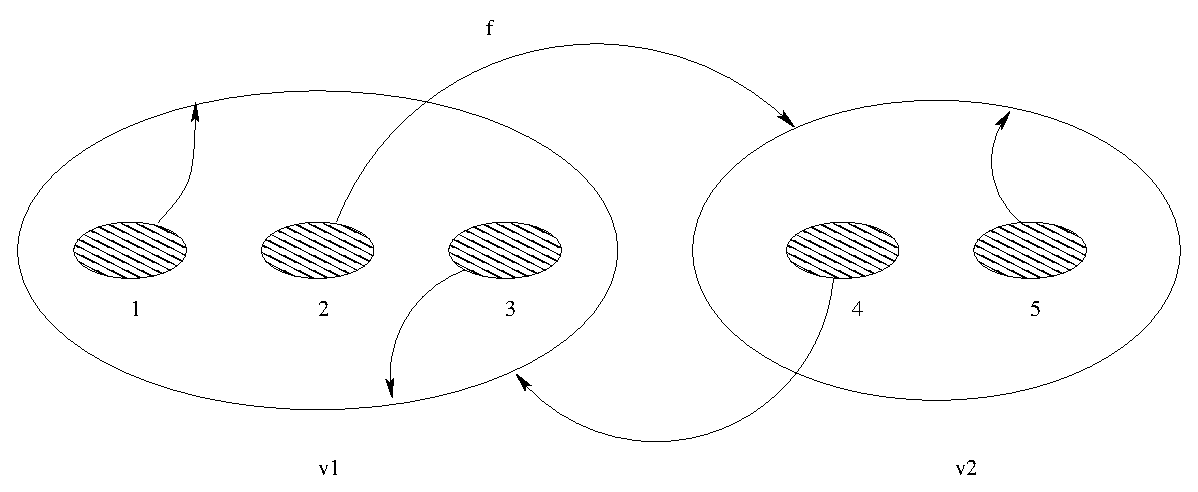
\includegraphics[width=18pc]{cantor1.eps}\\[17pt]%
    \hbox to0pt{\rule{\textwidth}{0.5pt}}\\%
    \hbox to0pt{\verb"  \begin{SCfigure}[50]"}\\[-2pt]%
    \hbox to0pt{\verb"    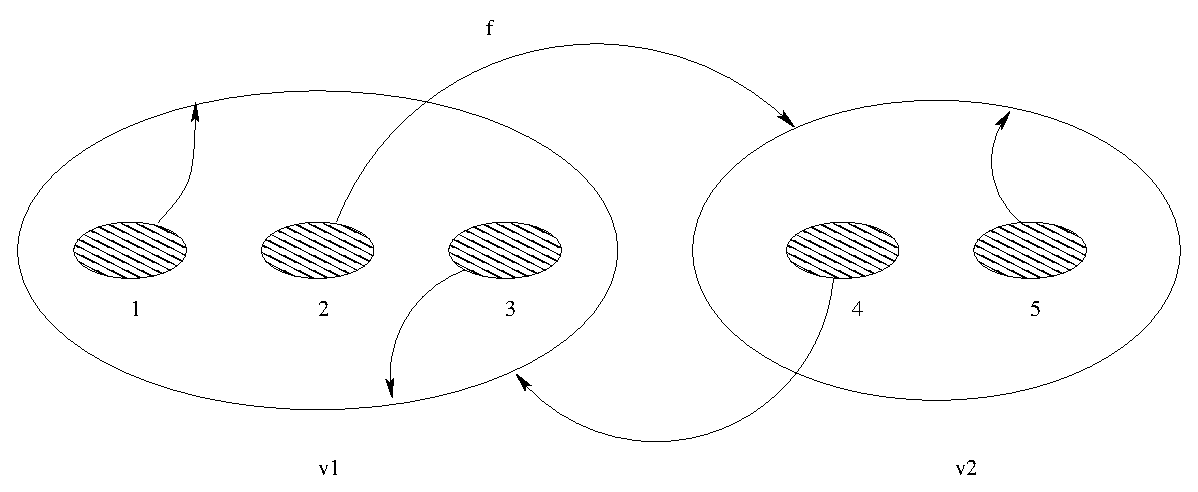
\includegraphics[width=18pc]{cantor1.eps}"}\\[-2pt]%
    \hbox to0pt{\verb"      \caption[Figure with side caption]"}\\[-2pt]%
    \hbox to0pt{\verb"        {The \texttt{SCfigure} environment should be used if you"}\\[-2pt]%
    \hbox to0pt{\verb"        would like a side caption.}"}\\[-2pt]%
    \hbox to0pt{\verb"      \label{scfigure}"}\\[-2pt]%
    \hbox to0pt{\verb"  \end{SCfigure}"}%
    \hbox to0pt{\rule[-10pt]{\textwidth}{0.5pt}}%
      \caption[Figure with side caption]
        {The \texttt{SCfigure} environment should be used if you
          would like a side caption.\vspace{119pt}}
      \label{scfigure}
  \end{SCfigure}


\subsection{Figures wider than the text width}

The \cambridge\ design will allow you to have figures exactly 33pc wide; these will extend into the left margin. For these, you would use the standard \texttt{figure} environment, but you need to add \verb"\widefigure" before the graphic is included, as shown in Figure~\ref{widefigure}.

  \begin{figure}
    \widefigure
    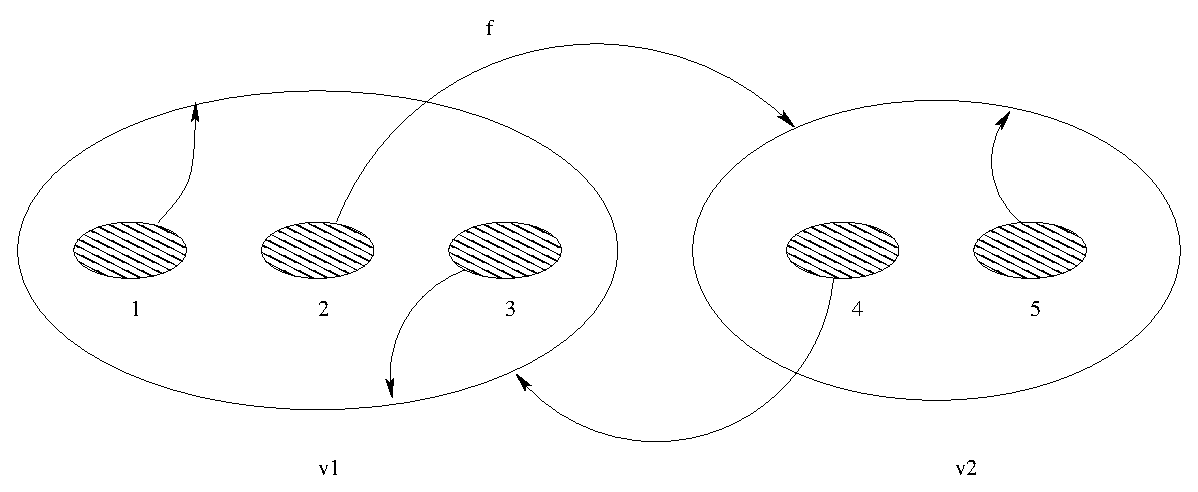
\includegraphics[width=33pc]{cantor1.eps}
    \caption[A wide figure]
      {Wide figures (33pc) may extend into the left-hand margin.}
    \label{widefigure}
\rule[-20pt]{\textwidth}{0.5pt}
\begin{verbatim}
  \begin{figure}
    \widefigure
    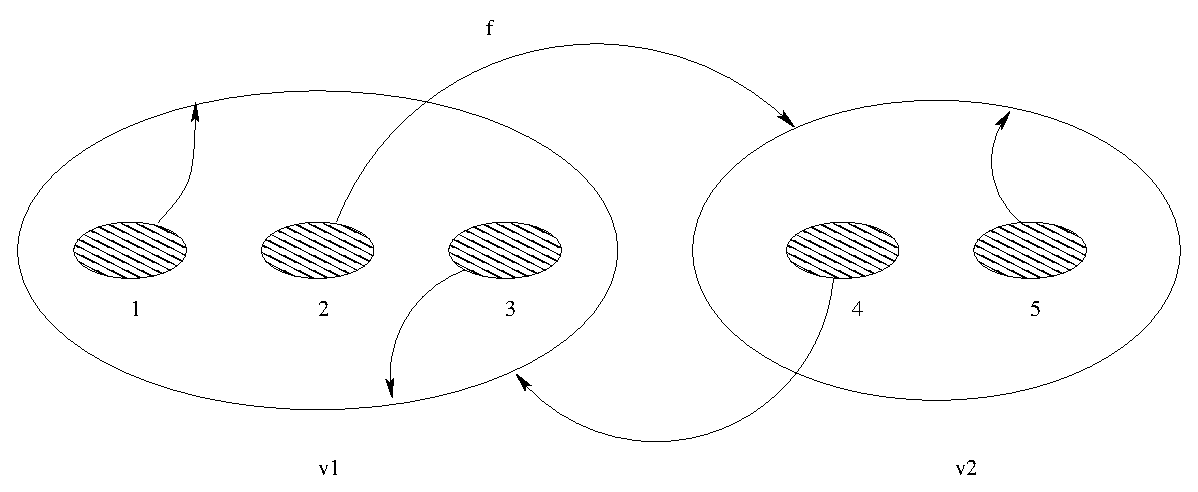
\includegraphics[width=33pc]{cantor1.eps}
    \caption[A wide figure]
      {Wide figures (33pc) may extend into the left-hand margin.}
    \label{widefigure}
  \end{figure}
\end{verbatim}
\rule[20pt]{\textwidth}{0.5pt}
  \end{figure}


\section{Tables}

The \cambridge\ class file will cope with most positioning of your tables. Tables need to be keyed slightly differently depending on their width. When you are first writing your book, assume that they will all be the full width of the page (see Section~\ref{overtwothirds}), and adjust this later.

As captions are normally positioned above tables, the caption must be included first, then the label, then the table. Note that if you are producing a list of tables (using \verb"\listoftables"), you need to repeat the caption in square braces, but without the full point.

Note that the \verb"\begin{tabular}{@{}lllllll@{}}" command always starts and finishes with \verb"@{}". This removes the space to the left of the first column, and to the right of the last column. You need to do this as the specification for tables in the \cambridge\ design is flush-left.

\subsection{Tables between two-thirds and full text width}
\label{overtwothirds}

If the width of the table lies between two-thirds and the full text width (in other words, between 19pc and 29pc), the table may be typeset using \verb"table*" (see Table~\ref{problimits}).

The \verb"table*" environment will give full-page width \verb"\hline"s; as a result you will most likely need to increase the space between columns to make the table fill the width of the page. If you are producing the final typeset version of your book, the space may be increased by changing \verb"\tabcolsep" as shown in Table~\ref{problimits}. If not, do not concern yourself with these values as they may change with a font substitution.

  \begin{table*}
    \caption[Probability left and right for the cost data]
      {Probability left and right of the exact confidence limits
      for the ratio of exponential means for the cost data.
      The exact limits were computed using the $F$~distribution and
      the approximate probability using the $r^*$ approximation.
      In this example, the Lugannani--Rice and $r^*$ approximations
      are identical.}
    \label{problimits}
    \addtolength\tabcolsep{4pt}% to stretch columns, if required
    \begin{tabular}{@{}lllllll@{}}
      \hline
      Exact
        & 0.20      & 0.10       & 0.05       & 0.025      & 0.001\\
      Approx. (left)
        & 0.199\,98 & 0.099\,992 & 0.049\,997 & 0.024\,999 & 0.0001\,000\\
      Approx. (right)
        & 0.200\,03 & 0.100\,239 & 0.050\,015 & 0.025\,009 & 0.0001\,000\\
      \hline
    \end{tabular}
\rule[-20pt]{\textwidth}{0.5pt}
\begin{verbatim}
  \begin{table*}
    \caption[Probability left and right for the cost data]
      {Probability left and right of the exact confidence limits
      for the ratio of exponential means for the cost data.
      The exact limits were computed using the $F$~distribution and
      the approximate probability using the $r^*$ approximation.
      In this example, the Lugannani--Rice and $r^*$ approximations
      are identical.}
    \label{problimits}
    \addtolength\tabcolsep{4pt}% to stretch columns, if required
    \begin{tabular}{@{}lllllll@{}}
      \hline
      Exact
        & 0.20      & 0.10       & 0.05       & 0.025      & 0.001\\
      Approx. (left)
        & 0.199\,98 & 0.099\,992 & 0.049\,997 & 0.024\,999 & 0.0001\,000\\
      Approx. (right)
        & 0.200\,03 & 0.100\,239 & 0.050\,015 & 0.025\,009 & 0.0001\,000\\
      \hline
    \end{tabular}
  \end{table*}
\end{verbatim}
\rule[20pt]{\textwidth}{0.5pt}
\end{table*}

\subsection{Tables less than two-thirds of the text width}

If you have a table which takes up less than two-thirds of the text width, i.e. less than 19pc, you have two options. You may either have the caption above the table, or choose the space-saving option of placing it to the side.

\subsubsection{Caption above table}

In this case, you would use the \verb"table" environment; see Table~\ref{piexample}.

  \begin{table}
    \begin{minipage}{160pt}
      %  note that the square brace option below is only required
      %  if you intend to produce a list of tables
    \caption[Shortened table caption for the list of tables]
      {Longer table captions have to be placed inside a minipage,
      otherwise they overhang the table rules.}
    \label{piexample}
    \addtolength\tabcolsep{2pt}% to stretch columns, if required
      \begin{tabular}{@{}c@{\hspace{25pt}}ccc@{}}
        \hline
        Figure\footnote{\textit{Note:} You must also use a minipage
          environment if you have footnotes.} & $hA$ & $hB$ & $hC$\\
        \hline
        1 & $\exp\left(\pi i\frac58\right)$
          & $\exp\left(\pi i\frac18\right)$ & $0$\\[3pt]
        2 & $-1$    & $\exp\left(\pi i\frac34\right)$ & $1$\\[11pt]
        3 & $-4+3i$ & $-4+3i$ & $\frac74$\\[3pt]
        4 & $-2$    & $-2$    & $\frac54 i$ \\
        \hline
      \end{tabular}
    \end{minipage}
\rule[-20pt]{\textwidth}{0.5pt}
\begin{verbatim}
  \begin{table}
    \begin{minipage}{160pt}
      %  note that the square brace option below is only required
      %  if you intend to produce a list of tables
    \caption[Shortened table caption for the list of tables]
      {Longer table captions have to be placed inside a minipage,
      otherwise they overhang the table rules.}
    \label{piexample}
    \addtolength\tabcolsep{2pt}% to stretch columns, if required
      \begin{tabular}{@{}c@{\hspace{25pt}}ccc@{}}
        \hline
        Figure\footnote{\textit{Note:} You must also use a minipage
          environment if you have footnotes.} & $hA$ & $hB$ & $hC$\\
        \hline
        1 & $\exp\left(\pi i\frac58\right)$
          & $\exp\left(\pi i\frac18\right)$ & $0$\\[3pt]
        2 & $-1$    & $\exp\left(\pi i\frac34\right)$ & $1$\\[11pt]
        3 & $-4+3i$ & $-4+3i$ & $\frac74$\\[3pt]
        4 & $-2$    & $-2$    & $\frac54 i$ \\
        \hline
      \end{tabular}
    \end{minipage}
  \end{table}
\end{verbatim}
\rule[20pt]{\textwidth}{0.5pt}
  \end{table}


\subsubsection{Caption to the side of table}

To typeset the table caption to the side, we recommend using the \verb"sidecap" style file; for coding see Table~\ref{sctable}. Note that the \verb"[50]" option on the first line will make the caption extend to the full width of the page, and is therefore essential.

Should you have a long caption which extends below the table, you will need to revert to the \verb"table" environment.

  \begin{SCtable}[50]
      \caption[Table with side caption]
          {The \texttt{SCtable} environment should be used if you
          would like a side caption. Measured and theoretical
          temperatures~($^\circ$C) in~20~sections of a reactor
          (Cox and Snell, 1981, Example~D).}
    \label{sctable}
    \begin{tabular}{@{}cc@{}}
      \hline
      Measured & Theoretical\\
      \hline
      431 & 432\\
      450 & 470\\
      431 & 442\\
      453 & 439\\
      481 & 502\\
      449 & 445\\
      441 & 455\\
      \hline
      \end{tabular}\\[13pt]
      \begin{tabular}{@{}p{0pt}@{}}
      \rule[2pt]{\textwidth}{0.5pt}\\
      \verb"  \begin{SCtable}[50]"\\
      \verb"    \caption[Table with side caption]"\\
      \verb"      {The \texttt{SCtable} environment should be used if you"\\
      \verb"      would like a side caption. Measured and theoretical"\\
      \verb"      temperatures~($^\circ$C) in~20~sections of a reactor"\\
      \verb"      (Cox and Snell, 1981, Example~D).}"\\
      \verb"    \label{sctable}"\\
      \verb"      \begin{tabular}{@{}cc@{}}"\\
      \verb"        \hline"\\
      \verb"        Measured & Theoretical\\"\\
      \verb"        \hline"\\
      \verb"        431 & 432\\"\\
      \verb"        450 & 470\\"\\
      \verb"        431 & 442\\"\\
      \verb"        453 & 439\\"\\
      \verb"        481 & 502\\"\\
      \verb"        449 & 445\\"\\
      \verb"        441 & 455\\"\\
      \verb"        \hline"\\
      \verb"      \end{tabular}"\\
      \verb"  \end{SCtable}"\\
      \rule[2pt]{\textwidth}{0.5pt}\\
    \end{tabular}
  \end{SCtable}

\subsection{My vertical rules have disappeared}

Vertical rules in tables are not \cambridge\ style, and have been automatically removed; this gives your document a truly professional look. Instead of vertical rules, we recommend the use of extra horizontal space, see Section~\ref{addhoriz}. The rules have been removed by redefining the \verb"tabular" environment. The amended definition also inserts extra vertical space above and below the horizontal rules (produced by \verb"\hline").

If you really must have them reinstated, read Section~\ref{reinstate}.

\subsection{Reinstating the vertical rules}
\label{reinstate}
Authors can revert to the standard \LaTeX\ style, if necessary. Tables will take on a rather squashed appearance, as in the \LaTeX\ book, whereby there is no added space around horizontal rules. Add the command \verb"\reinstaterules" in the preamble, and re-run your files through \LaTeX.

\subsection{There is very little space around the rules in my~table}
Tables revert to the standard, rather squashed look of standard \LaTeX\ tables for two reasons:
\begin{enumerate}
  \item you are using \verb"array.sty"; or
  \item you have chosen to reinstate vertical rules (see Section~\ref{reinstate})
\end{enumerate}
In both cases, the tabular environment is redefined.


\subsection{Adding space between columns}
\label{addhoriz}
You can add space (2pt in this example) between every column using\linebreak \verb"\addtolength\tabcolsep{2pt}". However, if you only wanted to expand the space between columns~1 and~2 to~25pt, you would do this using\linebreak \verb"\begin{tabular}{@{}c@{\hspace{25pt}}ccc@{}}" (see Table~\ref{piexample}).

\subsection{Adding space between rows}
If you need some form of separation between rows (for example, between rows~2 and~3 in the body of Table~\ref{piexample}), adding \verb"[11pt]" immediately after the double backslash at the end of row~2 will add a 11pt vertical space (the equivalent of a blank line at this typesize). This is neater than adding another horizontal line.


\section{Landscape figures and tables, using rotating.sty}

Landscape figures and tables (floats) may be typeset using the \verb"rotating.sty" package. Note that the direction of rotation depends on the page number -- which requires at least two passes through \LaTeX. If we are going to know whether pages are odd or even, we need to use the \verb"\pageref" mechanism, and labels. But labels won't work unless the user has put in a caption. \textit{Beware!}

In addition to \verb"rotating.sty", you should also include \verb"floatpag.sty" and the command \verb"\rotfloatpagestyle{empty}". This combination ensures that headers and footers are removed from the float page:
\begin{verbatim}
  \usepackage{rotating}
  \usepackage{floatpag}
  \rotfloatpagestyle{empty}
\end{verbatim}
In some DVI previewers, floats may not appear rotated. If this happens, you need to convert the DVI file to PostScript or PDF.

Occasionally, when you convert a PostScript file to a PDF file, you may find that the page comes out upside-down. There will be a setting to change this. For instance, if you are using PDFCreator 0.9.7, choose the following options in this sequence:
\begin{description}
  \item Options -- Program -- PDF -- Auto-Rotate Pages: Change to `None'.
\end{description}
Other programs will have similar procedures.

\subsection{Coding for landscape figures}

The landscape figure (Figure~\ref{sidecantor}) was typeset using the following coding:
\begin{verbatim}
  \begin{sidewaysfigure}
    \centering
    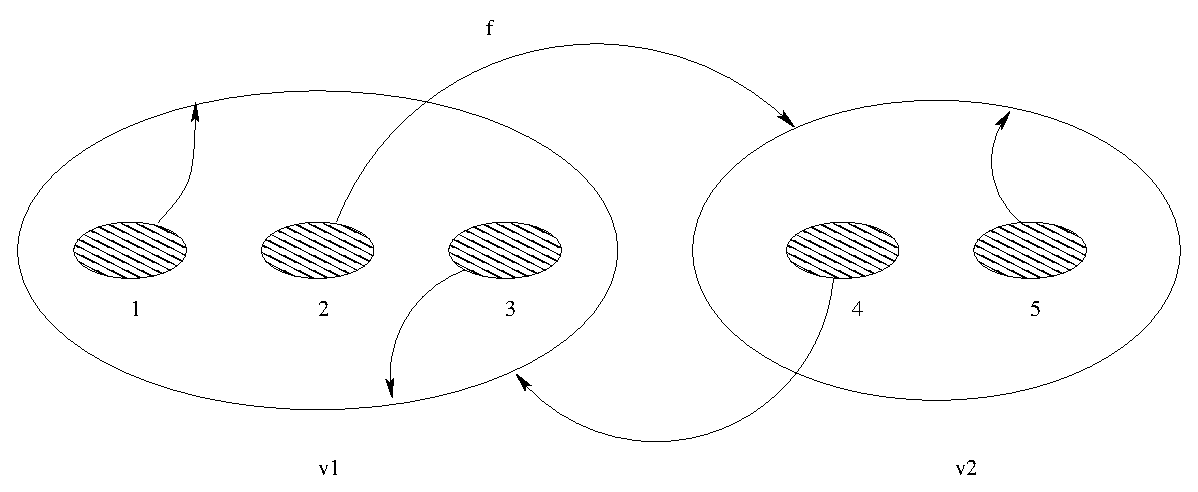
\includegraphics[scale=0.85]{cantor1.eps}
    %  note that the square brace option below is only required
    %  if you intend to produce a list of illustrations
    \caption[Landscape figure]{A Cantor repeller. Figure captions
      will be centred by default.}
    \label{sidecantor}
  \end{sidewaysfigure}
\end{verbatim}
  \begin{sidewaysfigure}
    \centering
    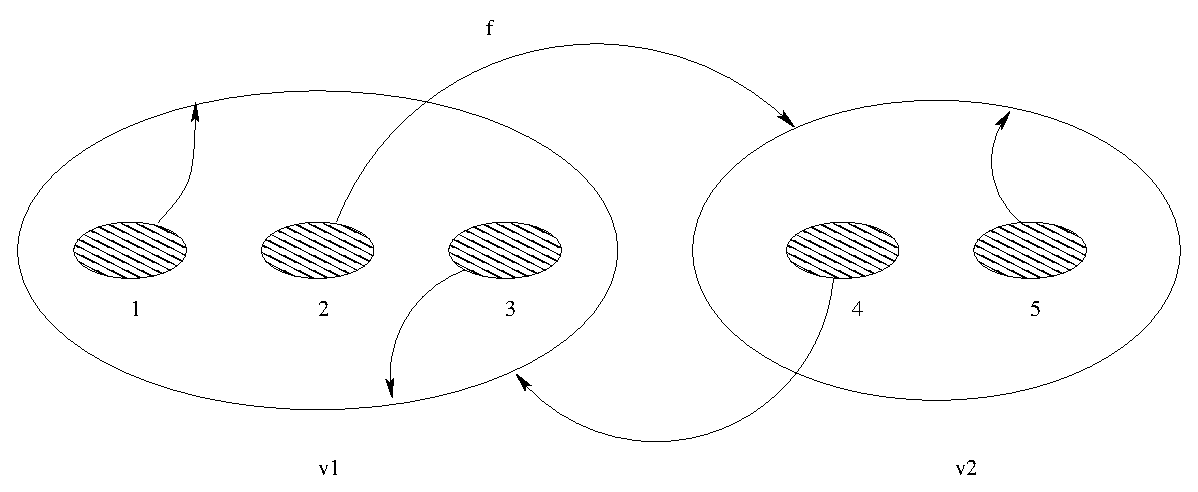
\includegraphics[scale=0.85]{cantor1.eps}
    %  note that the square brace option below is only required
    %  if you intend to produce a list of illustrations
    \caption[Landscape figure]{A Cantor repeller. Figure captions
      will be centred by default.}
    \label{sidecantor}
  \end{sidewaysfigure}


\subsection{Coding for landscape tables}

Table~\ref{sideways} has been produced using the following coding:
%
\begin{smallverbatim}
\begin{sidewaystable}
\begin{minipage}{465pt}
  \caption[Landscape table]{Grooved ware and beaker features, their finds and
    radiocarbon dates. For a breakdown of the pottery assemblages see
    Tables~I and~III; for the flints see Tables~II and~IV; for the animal
    bones see Table~V.}
  \label{sideways}
  \addtolength\tabcolsep{-2pt}
  \begin{tabular}{@{}lcccllccccc@{}}
  \hline
  Context & Length & Breadth/  & Depth & Profile & Pottery & Flint & Animal
                                                   & Stone & Other & C14 Dates\\
  && Diameter &&&&& Bones\\[5pt]
  & m & m & m\\
  \hline\\[-5pt]
  \multicolumn{10}{@{}l}{\textbf{Grooved Ware}}\\
  784 & --   & 0.9$\phantom{0}$ &0.18  & Sloping U & P1      & $\times$46
        & $\phantom{0}$$\times$8 && $\times$2 bone & 2150 $\pm$100\,\textsc{bc}\\
  785 & --   & 1.00             &0.12   & Sloping U & P2--4  & $\times$23
                                           & $\times$21 & Hammerstone & -- & --\\
  962 & --   & 1.37             &0.20   & Sloping U & P5--6  & $\times$48
                     & $\times$57 & --& --& 1990 $\pm$80\,\textsc{bc} (Layer 4)\\
  &&&&&&&&&& 1870 $\pm$90\,\textsc{bc} (Layer 1)\\
  983 & 0.83 & 0.73             &0.25   & Stepped U & --     & $\times$18
                                & $\phantom{0}$$\times$8 & -- & Fired clay & --\\
  &&&&&&&&&&\\
  \multicolumn{10}{@{}l}{\textbf{Beaker}}\\
  552 & --   & 0.68             & 0.12  & Saucer    & P7--14 & --           & --
                                                                   & -- &-- &--\\
  790 & --   & 0.60             & 0.25  & U         & P15    & $\times$12   & --
                                                      & Quartzite-lump & -- &--\\
  794 & 2.89 & 0.75             & 0.25  & Irreg.    & P16    & $\phantom{0}$$\times$3
                                                              & -- & -- &-- &--\\
  \hline
  \end{tabular}%
\end{minipage}
\end{sidewaystable}
\end{smallverbatim}
%
\begin{sidewaystable}
\begin{minipage}{465pt}
  \caption[Landscape table]{Grooved ware and beaker features, their finds and
    radiocarbon dates. For a breakdown of the pottery assemblages see
    Tables~I and~III; for the flints see Tables~II and~IV; for the animal
    bones see Table~V.}
  \label{sideways}
  \addtolength\tabcolsep{-2pt}
  \begin{tabular}{@{}lcccllccccc@{}}
  \hline
  Context & Length & Breadth/  & Depth & Profile & Pottery & Flint & Animal
                                                   & Stone & Other & C14 Dates\\
  && Diameter &&&&& Bones\\[5pt]
  & m & m & m\\
  \hline\\[-5pt]
  \multicolumn{10}{@{}l}{\textbf{Grooved Ware}}\\
  784 & --   & 0.9$\phantom{0}$ &0.18  & Sloping U & P1      & $\times$46
        & $\phantom{0}$$\times$8 && $\times$2 bone & 2150 $\pm$100\,\textsc{bc}\\
  785 & --   & 1.00             &0.12   & Sloping U & P2--4  & $\times$23
                                           & $\times$21 & Hammerstone & -- & --\\
  962 & --   & 1.37             &0.20   & Sloping U & P5--6  & $\times$48
                     & $\times$57 & --& --& 1990 $\pm$80\,\textsc{bc} (Layer 4)\\
  &&&&&&&&&& 1870 $\pm$90\,\textsc{bc} (Layer 1)\\
  983 & 0.83 & 0.73             &0.25   & Stepped U & --     & $\times$18
                                & $\phantom{0}$$\times$8 & -- & Fired clay & --\\
  &&&&&&&&&&\\
  \multicolumn{10}{@{}l}{\textbf{Beaker}}\\
  552 & --   & 0.68             & 0.12  & Saucer    & P7--14 & --           & --
                                                                   & -- &-- &--\\
  790 & --   & 0.60             & 0.25  & U         & P15    & $\times$12   & --
                                                      & Quartzite-lump & -- &--\\
  794 & 2.89 & 0.75             & 0.25  & Irreg.    & P16    & $\phantom{0}$$\times$3
                                                              & -- & -- &-- &--\\
  \hline
  \end{tabular}%
\end{minipage}
\end{sidewaystable}

\endinput